\documentclass{standalone}
\usepackage{tikz}

\begin{document}

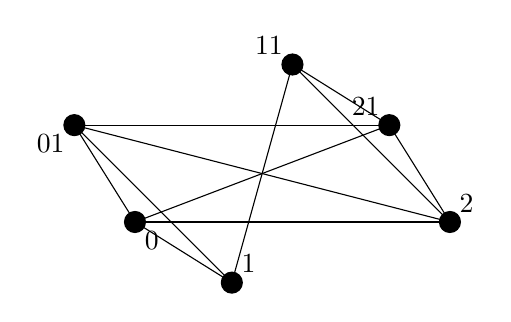
\begin{tikzpicture}[scale=2]
    % Define coordinates
    \coordinate (A) at (1,0,1);
    \coordinate (B) at (1,1,0);
    \coordinate (C) at (0,0,0);
    \coordinate (D) at (0,1,1);
    \coordinate (E) at (2,0,0);
    \coordinate (F) at (2,1,1);

    % Draw nodes
    \foreach \point in {A,B,C,D,E,F} {
        \fill (\point) circle (2pt);
    }

    % Label nodes
    \node[above right] at (A) {1};
    \node[above left] at (B) {11};
    \node[below right] at (C) {0};
    \node[below left] at (D) {01};
    \node[above right] at (E) {2};
    \node[above left] at (F) {21};

    % Draw edges
    \draw (A) -- (B);
    \draw (A) -- (C);
    \draw (A) -- (D);
    \draw (B) -- (E);
    \draw (B) -- (F);
    \draw (C) -- (D);
    \draw (C) -- (E);
    \draw (C) -- (F);
    \draw (D) -- (E);
    \draw (D) -- (F);
    \draw (E) -- (F);

\end{tikzpicture}

\end{document}